% !TEX root = ../thesis.tex

\chapter{Theory}
\label{sec:theory}

\cleanchapterquote{At the end of the century one will be able to speak of machines thinking without expecting to be contradicted.}{Alan Turing}{(Computing Machinery and Intelligence (1950))}

In this chapter I cover the basic concepts of Neural Networks that will be used later on when separation of style and content is discussed in more detail.
My intention is to allow anybody with basic knowledge in Mathematics and Computing to understand this manuscript from beginning to end.

The explanations will be developed from basic to complex so that a sequential read should guide the reader logically from question to answer while giving as much insight will be necessary to continue and just enough context to understand the raison d'être of the each concept.


% ------------------------------------------------------------------------------

\section{Background}
\label{sec:theory:background}

Before diving into technical aspects, however, I believe it is worth stopping to first introduce the fields of this thesis: \emph{Neural Networks} and \emph{Deep Learning}.
Neural Networks is an area of \emph{Machine Learning} very closely related with \emph{Cognitive Sciences} and Deep Learning is also an area of Machine Learning that typically uses neural networks, but let us go step by step.


\subsection{Neural Networks}
\label{sub:theory:background:neural-networks}

We can describe the field of Machine Learning as the study that enables computers to resolve problems for which they have not been explicitly programmed for by using some learning mechanism \citet{Samuel1959}.
When explicitly programming an algorithm to resolve a problem its complexity grows dramatically with that of the problem and the desired precision.
A perfectly robust algorithm that follows this approach will require: 1) the programmer to understand the problem completely so that all variables can be taken into account; 2) a hardware powerful enough to handle all these variables; and 3) data with maximum precision.
It is easy to see how one or more of these requirements will pose complications when the problem is complex enough.
Driving a car is a complex enough problem to make Classic Computing incapable of solving it.
Conversely, driving a car is a simple enough problem so that any person can do it.
The human mind can handle the task because, although not having perfect senses nor 100\% understanding on the laws of physics, how the car works, how other drivers exactly behave and many other factors involved; is capable of dealing with partial information, uncertainty, imprecision and approximations after having learned from experience \cite{Zadeh1994}.
Opposed to how Classic Computing tries to accurately model the world to solve problems, some fields of Machine Learning try to model how the human mind learns the complexity of the world to reason and act upon it.

At this point it is clear how the study of the human mind plays an important role in Machine Learning.
Cognitive Sciences is the field that studies the human mind and how it acquires understanding through experience and the senses.
Modern Cognitive Sciences have their inception in the 1940s, when efforts were being made to understand the principles of the mind by representing their structures and processes instead of operating directly on them \cite{Thagard2008}.
The studies quickly branched-off in 1943 when \citet{McCulloch1943}, inspired by biological neural networks, described the first mathematical model of an artificial neural network.
The field Neural Networks, shorthand for \emph{Artificial Neural Networks} (ANNs), quickly grew in the 1950s when they started being implemented \cite{Farley1954,Rosenblatt1958} as approximation or classification methods.

Since then, the field has evolved and expanded into a myriad of different methods that have maintained the purity with their biological counterparts in greater or lesser degree.
Within the general framework, we can still talk of neurons, organized in \emph{layers}, implementing an \emph{activation function} and storing experience in \emph{weights} as depicted in Figure~\ref{fig:sec:theory:neurons}.
An artificial neuron is a simple processing unit, forming networks typically organized in layers, whose input is the set of output of connected neurons from the previous layer and the process it performs is determined by the activation function.
The activation function can be implemented either as a threshold to be reached for the neuron to send an output or simply as a transformation of any sort of the input.
Lastly, experience in ANNs can be understood as connection strength between neurons in biological neural networks and this mechanism is implemented as a set of adaptive parameters, commonly called weights, that modifies the value of each input of the neuron \cite{Hinton1990}.

\begin{figure}[htb]
  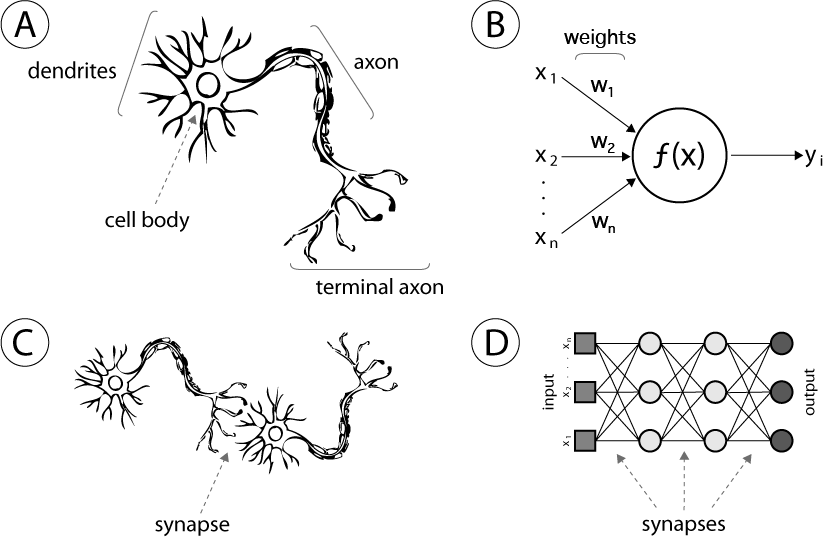
\includegraphics[width=\textwidth]{gfx/neurons}
  \caption{Biological Neuron vs Artificial Neuron \cite{Honorio2013}. AC) A biological neuron receives signals at the dendrites, the composition of the signals may or may not produce an excitation in the cell body based on experience, in which case a pulse will be transmitted down the axon and ultimately to other neurons' dendrites via terminal axon in a process called synapsis. BD) Similarly, artificial neuronal networks are organized in layers and synapsis occurs from layer to layer. An artificial neuron in the layer $Y$ receives one or more inputs $X$, representing dendrites, and result of an activation function $f(X)$ produces an output $y_i$, representing the axon, that gets passed to connected neurons in the subsequent layer. Weights represent connection strength between neurons and encode network experience.}
  \label{fig:sec:theory:neurons}
\end{figure}

A crucial step in preparing an ANN for a specific task is refining its set of weights.
That is what we refer to as training or supervised learning process.
Supervised learning is a data-driven process that requires a labeled training set of examples of which we know their class (dog vs. cat).
The process can be implemented in several ways but it generally boils down to defining some way to assess how far the prediction of the network is from an optimal solution, known as the \emph{loss function}, and the strategy that will propagate the error to refine the weights of the network.
Eventually, after enough training examples and corrections, the weights of the network will have adapted to generalize the features of the training data and will be more or less able to correctly classify new incoming examples.

The process can be seen as a teacher supervising the learning of a student.
The ``teacher" (loss function + weight rectification strategy) knows the correct solution (label of the example) and it corrects the ``student" (the network) when its prediction is incorrect.
An example of a completely wrong prediction would be the network having 100\% confidence of an image containing a dog when it clearly contains a cat.

One of the most important aspects that determines the accuracy of the network when presented with new examples is the volume of data and the correctness of its labels.
This becomes extremely important when trying to solve real-world problems like image recognition, where massive training sets are required to generalize networks for all concepts in a language under several different lighting conditions.
Big enough volumes of data have not been available until recently, and even nowadays, complete and accurately labeled datasets are expensive or time consuming to handcraft as the task may be too large or require expert knowledge on the specific field.
Approaches to work around this involved using partially labeled training datasets and pre-training the network first with unsupervised training where unlabeled examples with similar features are grouped together, then classified after the learning phase and finally used as additional training data \cite{Hinton2006}.
This approach is called semi-supervised learning and is one of the achievements of Deep Learning, which I am discussing next.


\subsection{Deep Learning}
\label{sub:theory:background:deep-learning}

Since 2006 the field of \emph{Deep Learning}, also called hierarchical learning, has appeared as a new area of Machine Learning research that brings it closer to its original goals: Artificial Intelligence \cite{Deng2014}.
Deep Learning focuses its efforts on producing methods for learning hierarchical feature representations, different levels of abstraction where higher-level ones are defined from lower-level ones, to help making sense of data such as images, sound and text in real-world applications.

One clear example of hierarchical representation is a spoken sentence.
A spoken sentence, the higher-level concept, is composed of spoken words.
A spoken word is made up of phonemes.
A phoneme is a representation of a speech sound with an associated waveform.
Making sense of speech in Deep Learning means first analyzing the waveform looking for phonemes, then trying to make up words from the phonemes found, and finally producing a grammatically correct and semantically meaningful sentence with those words.

As already mentioned in Chapter~\ref{sec:intro}, this kind of pattern recognition did not perform well until recently.
Traditional solutions employed shallow neural networks with simplistic models and limited representation power that could only be used to solve well-constrained problems like numerical approximations or binary classification.
Speech recognition, contrarily, is a very loosely-constrained problem and that is also the case for any problem dealing with the richness of data such as human voice, natural language and natural images.

Studies in human information processing mechanisms suggested the human brain uses deep neuronal architectures to extract complex patterns and build internal representations from rich sensory inputs.
For instance, the human speech perception system in the brain is equipped with layered hierarchical structures that transforms the information from the acoustic level to the linguistic level \cite{Deng1999,Baker2009}.
Training analogous deep architectures in artificial neural networks, \emph{deep neural networks} (DNNs), proved problematic from the beginning since classic learning algorithms tended to easily get trapped in poor local optima parameters.
This phenomenon, unfortunately, worsened quickly the more layers the neural network presented, which is the case of DNNs.

Efficient unsupervised learning algorithms that made use of the increasingly big datasets, available thanks to the widespread use of the Internet, were proposed to overcome the problems presented by local optima in classic learning algorithms \cite{LeCun2004,Hinton2006}, as previously discussed in Section~\ref{sub:theory:background:neural-networks}.
They, however, were so computationally expensive for training deep neural networks, having millions of parameters to learn, that were not widely used until parallelizable variations were proposed in 2012 \cite{Dean2012,Chen2012}.
These, alongside with powerful Graphic Processing Units (GPUs) becoming a commodity enabling the implementation of these algorithms marked the rapid expansion of Deep Learning in recent years.

Deep Learning is at the moment a quickly growing field covering a wide range of Machine Learning techniques and architectures.
In this thesis, I cover only the architecture of DNNs that we need for further discussing separation of style and content, Convolutional Neural Networks in Section~\ref{sec:theory:convnets}.
Before jumping too far ahead, the next sections of this chapter will go through the evolution of relevant ANNs architectures down from the most basic one, the Perceptron, up to the one at hand, Convolutional Neural Network.


% ------------------------------------------------------------------------------

\section{Perceptron}
\label{sec:Perceptron}
\todo[inline]{pattern recognition}

\begin{description}
  \item[Feed-forward Neural Networks]
  The simplest type of artificial neural network, characterized by its connections not forming cycles and thus the data always flowing in one direction: from input to hidden layers to output.
\end{description}
A perceptron is a type of cell that performs binary classification.

A binary classifier regardless of how it is implemented. It may very well be just a function or a whole deep neural network.

Weight
Also called learnable parameter or just parameter.
Coming from neuroscience literature, it refers to how much importance each one of the different input connections of a neuron has in the activation function.
\todo[inline]

\todo[inline]{Overfitting}

% ------------------------------------------------------------------------------

\section{Multilayer Perceptron}
\label{sec:theory:mlp}
A multilayer perceptron (MLP) is a type of feed-forward neural network composed of several layers where neurons of one layer are fully connected with the next one.
These neural networks are normally used to classify different inputs.

The limitations of the perceptron were mathematically proved \citet{Minsky1969} in 1969 and they claimed perceptrons with multiple layers would not be capable of solving not-linearly separable classes.
Discouraged by these claims little to none research was done in the field of Neural Networks until backpropagation was developed by \citet{Werbos1974}, rediscovered by \citet{Parker1985}, popularized by \citet{Rumelhart1988} and MLP were proved to be universal approximators \cite{Hornik1989,Ruck1990} in 1989.


\subsection{Backpropagation}
\label{sec:theory:mlp:backpropagation}
\todo[inline]


% ------------------------------------------------------------------------------

\section{Convolutional Neural Networks}
\label{sec:theory:convnets}
Convolutional Neural Networks, also known as CNNs or ConvNets, are feed-forward multi-layer neural networks inspired by cats' and monkeys' visual ventral stream \cite{Hubel1968,Lawrence1997} and are responsible for a major breakthroughs in image recognition \cite{LeCun1995}.
Before and contemporaneous to LeCun's LeNet \cite{LeCun1998} other networks like Fukushima's Neocognitron \cite{Fukushima1980} or Riesenhuber \& Poggio's HMAX \cite{Riesenhuber1999} were also inspired in the visual cortex, but it was the former that established the fundamentals for CNNs.
They are able to learn patterns in images from a training set through back-propagation and present built-in resilience towards translation and distortion variances in the input.
Such resilience minimizes pre-processing tasks both for training and classification and greatly reduces human supervision, making CNNs the currently preferred system for image recognition \cite{Visin2015}.

Although multi-layer perceptron are able to perform image recognition, they can only handle images of very small resolution due to the architectural limitations of fully connected layers \cite{ZHANG1999}.
Fully connected layers scale poorly, since neurons of the first hidden layer will process the whole image and will need to store weights for every color channel of every pixel.
Just to give a sense of the scale we are talking, for an RGB image of ${N}\times{M}$ pixels every neuron in a multi-layer perceptron will require storing ${N}\times{M}\times{3}$ weights, which for a ${32}\times{32}$ image it is $3072$ weights, but for a ${1024}\times{1024}$ one is more than $3$ millions.
In the shallower networks, with a single hidden layer, this already implies an exponential memory growth $O(N^2)$ with respect to image resolution.
Not only this is a performance issue in terms of hardware resources, the huge amount of parameters that need to be set also causes the system to quickly overfit.
Worse than that, treating pixels individually as described, regardless of their proximity, does not take into account the spatial information of an image.
That means that to handle variations in the images the network will end up with the same weights being stored in different neurons, proving multi-layer perceptron clearly inefficient for image recognition.
These problems are addressed by CNN architectural features \cite{LeCun1998}: 1) local receptive fields, 2) shared weights, and 3) subsampling.


\subsection{Properties}
\label{sub:concepts:convnets:properties}

\paragraph{Local receptive fields}
The term \emph{receptive field} is borrowed from the literature of neuroscience and it refers to an area of the body surface that trigger a neurological response in the presence of stimuli \cite{Sherrington1906,Alonso2008}.
In the context of convolution networks, receptive field refers to a region of the visual input, represented by an image, that is connected with one or several neurons that will react to it and is commonly called \emph{filter}.
Using local receptive fields means that neurons in the network will not react to the whole image but to a small region of it instead.
This ensures neurons will extract first the most basic visual features such as edges, end-points or corners;
In subsequent layers, from those elementary visual features, neurons will then extract progressively higher-order features like shapes, textures, faces or objects.
Such architecture allows effectively takes into account the spatial correlation existing in images.
Within a layer several neurons performing different feature detections can can be stacked to receive the input from the perceptive field as depicted in Figure~\ref{fig:sec:theory:conv-layer-1}.

\begin{figure}[htb]
  \begin{center}
    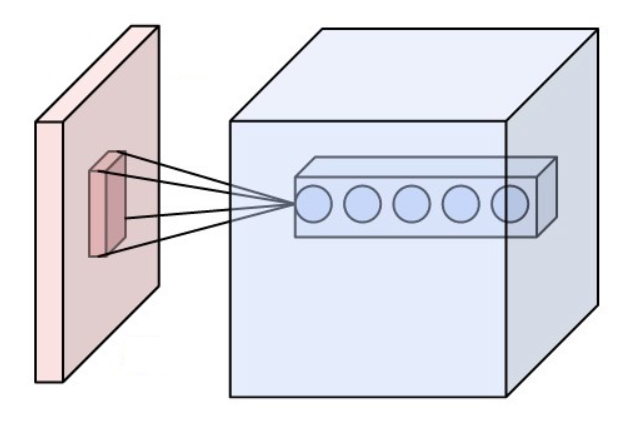
\includegraphics[width=0.6\textwidth]{gfx/conv-layer-1}
  \end{center}
  \caption{Stack of neurons applying different feature detections within a convolutional layer on the same perceptual region \cite{Aphex342015}.}
  \label{fig:sec:theory:conv-layer-1}
\end{figure}

\paragraph{Shared weights}
Layers in CNNs are organized in several slices, each of them containing neurons that detect the same feature but in different regions of the image and each slice detecting different features.
This operation is equivalent to a convolution in image processing, a sliding window that applies a transformation the original image, and that is where CNNs receive their name.
The sliding window is called kernel, filter or mask, and it is an image transformation matrix, usually small, that performs the weighted sum over a set of pixels of the original image, as shown in Figure~\ref{fig:sec:theory:kernel}
In this analogy, the kernel of the convolution is the filter applied by the slice over the input, represented by \emph{weights shared} by all its neurons, being this what makes feature recognition robust against translations or distortions in the image.
The output of the convolution is referred to as \emph{feature map}, and all feature maps produced by a convolutional layer together become the input for the next layer, usually called \emph{volume} since it has height, width and depth.
The height and width are proportional to the size of the original image and depth equal to the amount of slices in the layer.
Such architecture is depicted in Figure~\ref{fig:sec:theory:conv-layer-2}.

\begin{figure}[htb]
  \begin{center}
    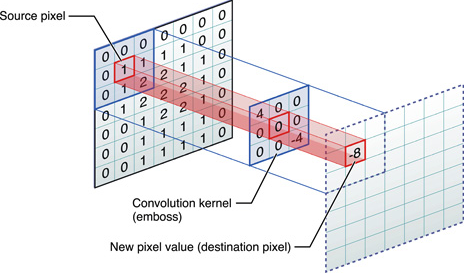
\includegraphics[width=0.5\textwidth]{gfx/kernel}
  \end{center}
  \caption{Convolutional kernel \cite{Apple}. The kernel gets centered on the source pixel and the convolution takes into account nearby pixels transforming the source pixel value. The convolution operation is a weighted sum of the source pixel with its nearby pixels. In this case:\\
    $(0\cdot4)+(0\cdot0)+(0\cdot0)
     +(0\cdot0)+(1\cdot0)+(1\cdot0)
     +(0\cdot0)+(1\cdot0)+(2\cdot-4) = -8$
  }
  \label{fig:sec:theory:kernel}
\end{figure}

\begin{figure}[htb]
  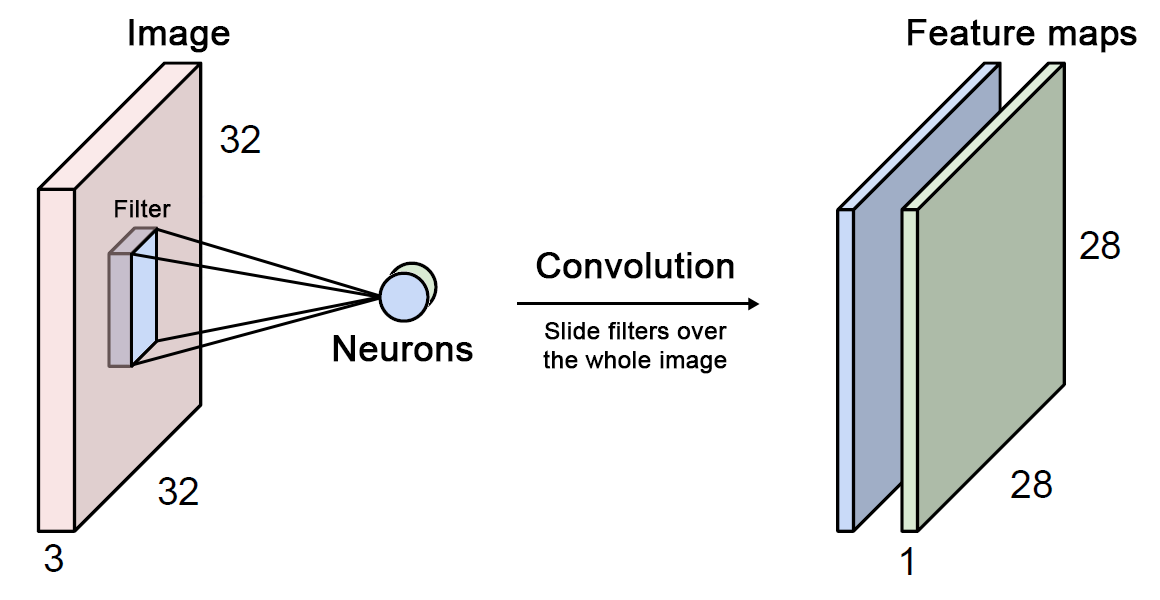
\includegraphics[width=\textwidth]{gfx/conv-layer-2}
  \caption{Anatomy of a convolutional layer and its output \cite{Guerzhoy2016}. On the left there is the representation of an image of ${32}\times{32}$ pixels with $3$ channels (\emph{RGB}). Neurons apply a filter of size ${5}\times{5}\times{3}$ in particular region of the image. Neurons of the same color belong to the same slice apply the same filter in different regions of the image and produce a feature map. All feature maps combined become the "new image" of size ${28}\times{28}\times{N}$, being $N$ the number of slices in the layer, that gets fed to the next layer.}
  \label{fig:sec:theory:conv-layer-2}
\end{figure}

\paragraph{Subsampling}
In the process of detecting higher-order features throughout subsequent layers of the network the exact absolute position of detected features in feature maps is pretty much irrelevant compared to the relative position between them.
For instance, the pattern that describes the number $7$ is an endpoint in upper left area of a horizontal segment, a corner in the upper right area and an endpoint at the bottom of a vertical segment.
Still, small variations in the input may cause the pattern not to be detected because the features will not completely match the filter.
To make the network more robust against variations the sensitivity of the convolutional layers has to be reduced.
This is effectively accomplished by reducing the resolution of the feature maps through non-linear \emph{subsampling} with pooling layers.
$Max$ is normally used as the non-linear function, giving the name of the subsampling operation \emph{max-pooling}, but it is not limited to it, as we will see in Chapter~\ref{sec:system}.
A pooling layer takes as input a volume of feature maps and, usually, has a non-overlapping filter of size ${2}\times{2}$ that gets applied on each one of the feature maps individually, as can be appreciated in Figure~\ref{fig:sec:theory:pooling}.
More specifically, the filter summarizes the feature map by performing max-pooling over its ${2}\times{2}$ regions and producing a single value for each, being this a size reduction of $75\%$.
It is important to note that this reduction applies only to the height and width of the original input since the depth refers to the amount of feature maps and these are preserved.

\begin{figure}
  \begin{subfigure}[b]{0.35\textwidth}
    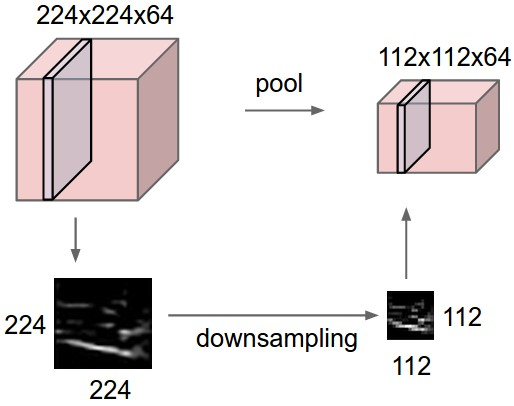
\includegraphics[width=\textwidth]{gfx/pool}
    \captionsetup{justification=centering}
    \caption{General pooling}
    \label{fig:sec:theory:pooling:general}
  \end{subfigure}
  \hfill
  \begin{subfigure}[b]{0.55\textwidth}
    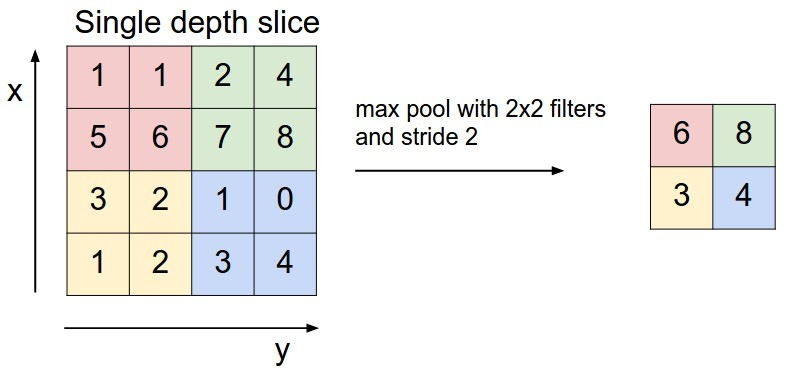
\includegraphics[width=\textwidth]{gfx/maxpool}
    \captionsetup{justification=centering}
    \caption{Max-pooling}
    \label{fig:sec:theory:pooling:max}
  \end{subfigure}
  \caption{Overview of a pooling layer. On the left, the input and output of a pooling layer reducing only the height and width of the volume \cite{Karpathy}. On the right, a single feature map of the input volume being subsampled by non-overlapping ${2}\times{2}$ max-pooling \cite{Karpathya}.}
  \label{fig:sec:theory:pooling}
\end{figure}


\subsection{Architecture}
\label{sub:concepts:convnets:achitecture}

While discussing the properties of ConvNets I have introduced two of their building blocks: convolutional layers and pooling layers.
These alone are not enough to use ConvNets for object recognition tasks since feature extraction is not the same as classification.
Let us have a look at how they fit in the big picture and the rest of the building blocks.

In Figure~\ref{fig:sec:theory:convnet} I present the typical configuration of a complete convolutional network.
We can see convolutional layers are alternated with pooling layers and ultimately fed into a fully connected network.
Whereas convolutional layers typically increase the amount of feature maps increasing the richness of intermediate representations, pooling layers reduce their spatial resolution keeping the amount of parameters low and thus limiting overfitting.
After several convolutional-pooling layers, the set of all feature maps, a highly abstracted representation the original image at that point, gets fed into fully connected layers, usually in the shape of a multilayer perceptron.
It is within the fully connected network that the classification takes place.

\begin{figure}[htb]
  \begin{center}
    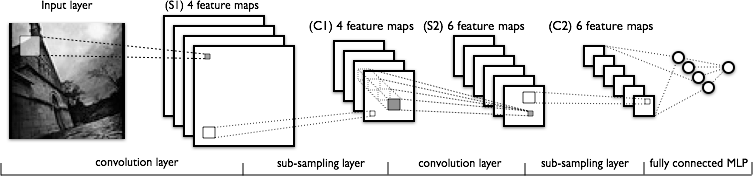
\includegraphics[width=\textwidth]{gfx/conv-network}
  \end{center}
  \caption{LeNet typical architecture \cite{LaboratoiredInformatiquedesSystemesAdaptatifs2010}. On the left there is an image (input layer). The image gets processed by a convolutional layer that extracts 4 elementary features producing 4 feature maps (S1). A pooling layer reduces the dimensionality while maintaining the same amount of feature maps (C1). Next, another convolutional layer extracts 6 higher-order features from the 4 feature maps (C2). Again, another pooling layer reduces the resolution of the 6 feature maps (S2). Finally, a fully-connected network takes the 6 feature maps and performs classification over them.}
  \label{fig:sec:theory:convnet}
\end{figure}

Additionally to these fundamental layers, normalization layers have been used as well.
These, however are \todo{cite}{falling out of use} since their contribution to the final result is close to none and they increase the complexity of the network.
ReLU \cite{Krizhevsky2012,Nair2010}

% It's important to note that all the weights in the network are learnt through back-propagation.

% One last element essential in convolutional networks is the loss layer.
% This layer calculates the error of the classifications


\todo[inline]{TODO}
Summarizing, CNNs are mainly composed by \todo{?}N types of layers: Convolutional layers, pooling layers, ReLU layers, fully connected layers.
Convolutional layers perform feature detection.
Pooling layers reduce the dimensionality of feature maps.
ReLU layers \todo{?}?.
Fully connected layers perform classification.

\paragraph{Feature learning}
Finding kernel that produce the desired feature maps is very difficult since it greatly varies depending on the task.
In CNN, feature learning is the step in which the kernel gets increasingly better at the task of filtering an image or a feature map coming from a previous layer.
\todo[inline]

\subsection{Hyperparameters}
\label{sub:concepts:hyperparameters}

It's worth noting that filters are always applied over the whole depth so that a ${W}\times{H}$ filter


% ------------------------------------------------------------------------------

\section{Convolutional Network Visualization}
\label{sec:theory:netvis}


% ------------------------------------------------------------------------------

\section{Adversarial Networks}
\label{sec:theory:adversarialnet}


% ------------------------------------------------------------------------------

\section{Non-linear transformations}
\label{sec:Non-linear transformations}

They are filters (a.k.a. kernel or feature map), often represented by $\phi$, implemented as functions whose output is not linear to its input often used for feature extraction on images (edges, connectivity, etc.). Perceptron neurons use these as activation function because the dimensionality of the input can be reduced so that it becomes binary classifiable.

\begin{description}
  \item[tanh]
  \item[ReLU]
\end{description}
